\documentclass[11pt]{article}
\usepackage[a4paper,margin=2cm]{geometry}
\title{%
    The Hare and the Tortoise \\
    \large A mini project \\
}
\author{Patrick Pellacani Muller}
\setcounter{section}{-1}

\usepackage{siunitx}
\usepackage{minted}

% tikz setup
\usepackage{tikz}
\usetikzlibrary{positioning,shapes.geometric,arrows.meta}

\tikzstyle{startstop} = [rectangle, rounded corners, minimum width=3cm, minimum height=0.8cm, text centered, draw=black, fill=gray!20, font=\small]
\tikzstyle{process} = [rectangle, minimum width=3cm, minimum height=0.8cm, text centered, draw=black, fill=gray!10, font=\small]
\tikzstyle{decision} = [diamond, aspect=2, text centered, draw=black, fill=gray!10, font=\small, inner sep=3pt]
\tikzstyle{io} = [trapezium, trapezium left angle=70, trapezium right angle=110,
                   minimum width=3cm, minimum height=0.8cm, text centered, draw=black, fill=gray!10, font=\small]
\tikzstyle{subprog} = [
    rectangle, minimum width=3cm, minimum height=0.8cm,
    text centered, draw=black, fill=gray!5, font=\small,
    inner xsep=8pt,
    path picture={
        \draw[line width=0.8pt] 
            ([xshift=0.15cm]path picture bounding box.north west) -- 
            ([xshift=0.15cm]path picture bounding box.south west);
        \draw[line width=0.8pt] 
            ([xshift=-0.15cm]path picture bounding box.north east) -- 
            ([xshift=-0.15cm]path picture bounding box.south east);
    }
]
\tikzstyle{arrow} = [thick, ->, >=Stealth]



\usepackage{datetime}
\newdate{writing_date}{13}{10}{2025}
\date{\displaydate{writing_date}}

\usepackage{biblatex}
\addbibresource{sources.bib}

\begin{document}
    \maketitle
    \section{Introduction}
    \subsection{Purpose}
    The main purpose of the program is entertainment as it is a game to be enjoyed. It
    simulates the classic story of the tortoise and the hare. To make the game enjoyable,
    the user is asked to bet on either the hare or the tortoise
    \subsection{Intended user}
    Possible users of the program are younger children as the game loop is very simple and
    may not appeal as much to older children, teenagers or adults. It should therefore be easy
    to use and understand.
    \subsection{Functionality}
    A simple pseudo-random number generator based simulation of the game of ``the hare and the
    tortoise''. The initial parameters for the simulation are:
    \begin{itemize}
        \item The game is divided into rounds, and finishes when the first person reaches
            \qty{1000}{\metre}
        \item Each round the tortoise moves \qtyrange{5}{10}{\metre}
        \item Each round the hare moves \qtyrange{8}{15}{\metre}
        \item However, there is a \qty{25}{\percent} chance that the hare doesn't move
    \end{itemize}

    \subsection{Why a computational approach was used}
    \label{sec:approach}
    A computational approach is best here as the races can be quite long and can be simulated more
    quickly. Therefore the user can run more simulations and the betting element (which is 
    the main engagement device) is more prominent.

    The programming language that is used in this project is Rust \cite{rust} which provides a 
    safe, compiled language. The main reasons for this is to offer security and help with data
    validation. By having using a compiled language, the program will run more efficiently, which
    isn't a major concern right now but allows for a better integration of a more complex UI and 
    game mechanic later. Furthermore, the game is aimed at children who often do not have the money
    to buy powerful PCs, and performance could be a major factor later on.

    \section{Data structures}
    The constants used in the program are defined in Table~\ref{tab:consts}, and the variables
    in Table~\ref{tab:vars}. Three custom structs are used for modularity, and their relationship as
    well as structure can be seen in Figure~\ref{fig:structs}.

    \begin{table}[!ht]
        \centering
        \begin{tabular}{ | c c | }
            \hline
            Name & type \\
            \hline
            \texttt{race\_length} & \texttt{u32} \\ 
            \texttt{tortoise\_speed\_interval} & \texttt{Interval} \\
            \texttt{hare\_speed\_interval} & \texttt{Interval} \\
            \texttt{hare\_sleep\_chance} & \texttt{f64} \\
            \hline
        \end{tabular}
        \caption{Constants used in the game}%
        \label{tab:consts}
    \end{table}
    \begin{table}[!ht]
        \centering
        \begin{tabular}{ | c c | }
            \hline
            Name & type \\
            \hline
            \texttt{hare} & \texttt{Hare} \\ 
            \texttt{tortoise} & \texttt{Tortoise} \\
            \texttt{winners} & \texttt{WinnerTable} \\
            \texttt{money} & \texttt{i32} \\
            \texttt{bet} & \texttt{Bet} \\
            \hline
        \end{tabular}
        \caption{Variables used in the game}
        \label{tab:vars}
    \end{table}

    \begin{figure}[!ht]
    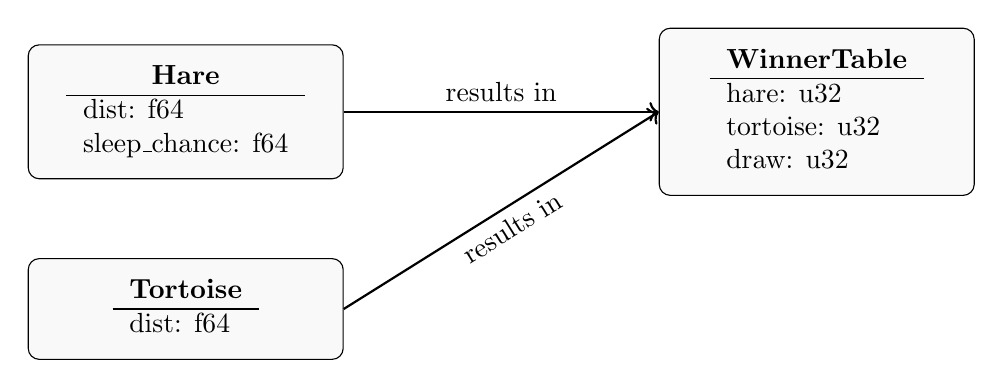
\begin{tikzpicture}[
    struct/.style={
        rectangle,
        draw=black,
        rounded corners,
        fill=gray!5,
        minimum width=4cm,
        inner sep=6pt
    },
    title/.style={
        fill=gray!20,
        font=\bfseries,
        text centered
    },
    field/.style={
        font=\ttfamily\small,
        anchor=west
    }
    ]

    % Hare struct
    \node[struct] (hare) {
    \begin{tabular}{l}
        \multicolumn{1}{c}{\textbf{Hare}} \\ \hline
        dist: f64 \\
        sleep\_chance: f64 \\
    \end{tabular}
    };

    % Tortoise struct
    \node[struct, below=of hare] (tortoise) {
    \begin{tabular}{l}
        \multicolumn{1}{c}{\textbf{Tortoise}} \\ \hline
        dist: f64 \\
    \end{tabular}
    };

    % WinnerTable struct
    \node[struct, right=4cm of hare] (winner) {
    \begin{tabular}{l}
        \multicolumn{1}{c}{\textbf{WinnerTable}} \\ \hline
        hare: u32 \\
        tortoise: u32 \\
        draw: u32 \\
    \end{tabular}

    };

    
    \draw[->, thick] (hare.east) -- node[above,sloped]{results in} (winner.west);
    \draw[->, thick] (tortoise.east) -- node[below,sloped]{results in} (winner.west);
    \end{tikzpicture}
    \caption{The structure diagram of the \texttt{struct}s \texttt{Hare}, \texttt{Tortiose} 
    and \texttt{WinnerTable}}
    \label{fig:structs}
    \end{figure}

    \section{Outline of Program}
    \subsection{Overview of main algorithm}
    The flowchart in Figure~\ref{fig:flw-prgm} outlines clearly the main program loop and how the main 
    part of the program calls the smaller modules. Below, the same idea, written in pseudocode, can be found.
    \begin{listing}
        \begin{minted}[frame=lines]{text}
        DO
            bet := setup_bet(Input("How much to bet?"), Input("Betting on tortoise or hare"))
            WHILE NOT race_ended()
                move_animals()
            ENDWHILE
            announce_winner()
            store_winner()
            calculate_bet()
        WHILE Input("Another Race?")
        output_stats()
        \end{minted}
        \caption{A pseudocode overview of the main program.}
        \label{lst:psd-overview}
    \end{listing}
    \begin{figure}[!ht]
        \centering
        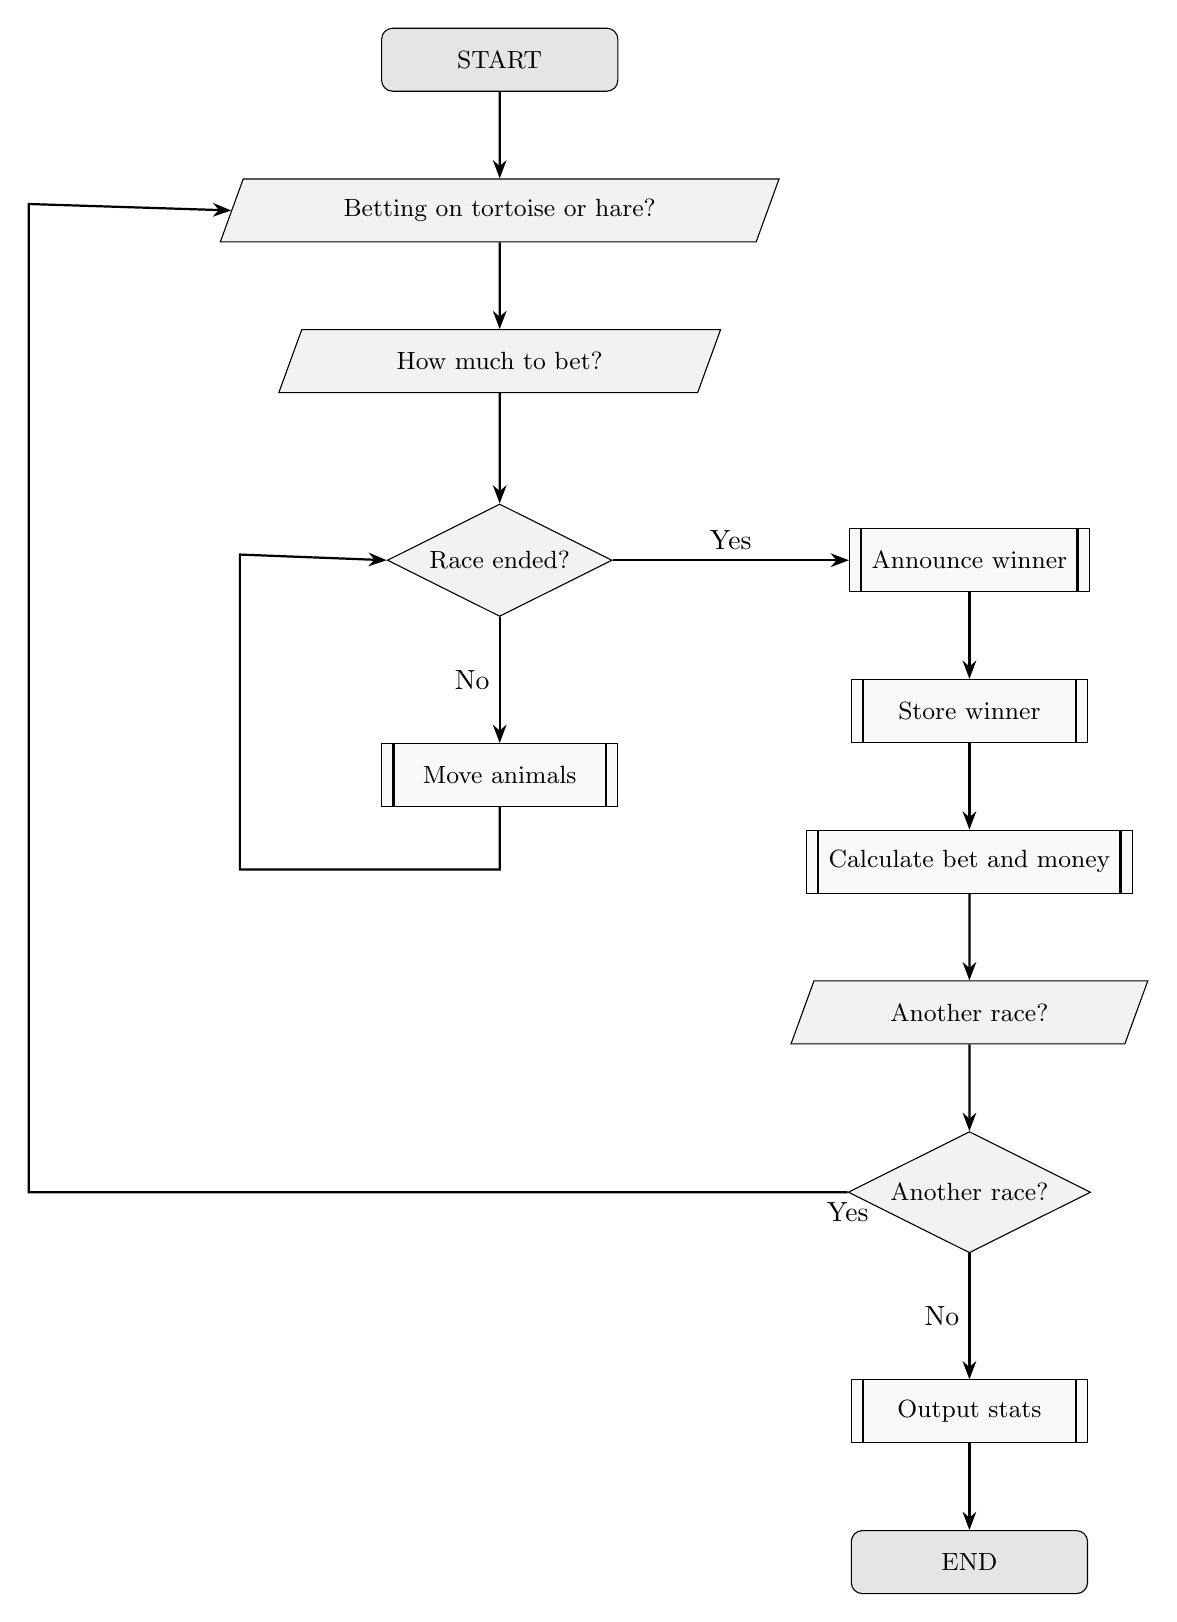
\begin{tikzpicture}[node distance=1.1cm]

            % Nodes
            \node (start) [startstop] {START};
            \node (betchoice) [io, below=of start] {Betting on tortoise or hare?};
            \node (betamt) [io, below=of betchoice] {How much to bet?};

            \node (racecheck) [decision, below=of betamt, yshift=-0.3cm] {Race ended?};
            \node (move) [subprog, below=of racecheck, yshift=-0.5cm] {Move animals};

            \node (announce) [subprog, right=3cm of racecheck] {Announce winner};
            \node (store) [subprog, below=of announce] {Store winner};
            \node (money) [subprog, below=of store] {Calculate bet and money};

            \node (again) [io, below=of money] {Another race?};
            \node (againcheck) [decision, below=of again] {Another race?};

            \node (stats) [subprog, below=of againcheck, yshift=-0.5cm] {Output stats};
            \node (stats) [subprog, below=of againcheck, yshift=-0.5cm] {Output stats};
            \node (stop) [startstop, below=of stats] {END};

            % Arrows
            \draw [arrow] (start) -- (betchoice);
            \draw [arrow] (betchoice) -- (betamt);
            \draw [arrow] (betamt) -- (racecheck);

            \draw [arrow] (racecheck) -- node[anchor=east] {No} (move);
            \draw [arrow] (move) -- ++(0,-1.2) -| ++(-3.3,4) -- (racecheck.west);
            \draw [arrow] (racecheck) -- node[anchor=south] {Yes} (announce);

            \draw [arrow] (announce) -- (store);
            \draw [arrow] (store) -- (money);
            \draw [arrow] (money) -- (again);
            \draw [arrow] (again) -- (againcheck);

            \draw [arrow] (againcheck) -- node[anchor=east] {No} (stats);
            \draw [arrow] (stats) -- (stop);
            \draw [arrow] (againcheck.west) node[anchor=north] {Yes} -- ++(-10.4,0) -- ++(0,12.55) -- (betchoice.west);
        \end{tikzpicture}
        \caption{Flowchart of the main program}
        \label{fig:flw-prgm}
    \end{figure}
    \subsection{Modularity}
    \label{sec:modules}

    \section{Test data}
    \subsection{Inputs and testing approach}
    The main data inputs are:
    \begin{itemize}
        \item Choosing between betting on the tortoise or hare
        \item Entering the amount of money to bet
        \item Deciding whether or not to play another round
    \end{itemize}

    Because Rust is used as the programming language (see Section~\ref{sec:approach}), data safety
    and errors such as buffer overflow errors are dealt with by the language. However, testing that
    these safeguards are in place properly is still good practice, especially as the default response
    to such an error in Rust would be a ``\texttt{panic}'', which stops the program abruptly and may
    instill annoyance in users if they experience such an error in the middle of the game.

    To ensure the correct functionality of individual modules, unit testing will be used throughout 
    the development phase. This ensures that the individual modules outlined in Section~\ref{sec:modules}
    are working as intended. The that is used for testing is outlined in Section ~\ref{sec:unit-test} 

    Furthermore, testing after development with valid, boundary, invalid and erroneous data will ensure 
    that the whole program works as expected. This data is outlined in Section~\ref{sec:whole-test}.
    \subsection{Unit Testting}
    \label{sec:unit-test}
    \subsection{Validation Testing}
    \label{sec:whole-test}
    \section{Source code}
    \section{Testing}
    \section{Evaluation}
\end{document}